% 5-page ACL paper. Independent of ../talk_like_a_graph.tex, which is not
% modified by anything in this directory.
%
% Build from this directory so the shared style/bib resolve:
%   cd paper/short && TEXINPUTS=..: BIBINPUTS=..: latexmk -pdf short.tex
%
% Every number traces to a script: see NUMBERS.md.
\documentclass[11pt]{article}
\usepackage[preprint]{acl}

\usepackage{times}
\usepackage{latexsym}
\usepackage[T1]{fontenc}
\usepackage[utf8]{inputenc}
\usepackage{microtype}
\usepackage{amsmath}
\usepackage{graphicx}
\usepackage{booktabs}
\usepackage{multirow}

\newcommand{\ncThirtyNinepOne}{98\%}
\newcommand{\ncThirtyNinepTwo}{100\%}
\newcommand{\ncThirtyNinepThreeFive}{72\%}
\newcommand{\ncThirtyNinepFive}{4\%}
\newcommand{\ecRelOneSevenbpOne}{16.5\%}
\newcommand{\ecRelOneSevenbpTwo}{43.0\%}
\newcommand{\ecRelOneSevenbpThreeFive}{22.8\%}
\newcommand{\ecRelOneSevenbpFive}{26.1\%}
\newcommand{\ecRelFourbpOne}{8.1\%}
\newcommand{\ecRelFourbpTwo}{9.7\%}
\newcommand{\ecRelFourbpThreeFive}{12.6\%}
\newcommand{\ecRelFourbpFive}{17.2\%}


\title{What GraphQA Measures at $n{=}40$, and What Structural Primers
Add to It}

\author{
  Gal Barak \\
  \footnotesize\texttt{github.com/GalBrk} \\\And
  Nitzan Zacharia \\
  \footnotesize\texttt{github.com/NitzanZacharia} \\\And
  Inbal Moryles \\
  \footnotesize\texttt{github.com/iinbal} \\
}

\begin{document}
\maketitle

\begin{abstract}
Prepending a \emph{primer} of factual sentences about a graph's structure to
its text encoding is a natural way to help a language model answer
graph-reasoning questions. We evaluate primers on six GraphQA tasks over
$40$-node Erd\H{o}s--R\'enyi graphs with four Qwen3 arms, against four
controls applied jointly: a graph-blind solver refit at the evaluated graph
size, a length-matched content-free filler, a minimal-length content control,
and the majority-class baseline of each task. Reading accuracy against the
class prior rather than against zero reorganises the benchmark: two of the six
tasks have a prior of $1.000$ at this graph size, and on a third both plain
arms score below the prior at every density. Within what remains, primers act
through two mechanisms. A primer that states the requested quantity is a
second route to the answer, helping a model at floor and harming one at
ceiling (cross-fitted interaction $-11.0$ points, $95\%$ CI $[-17.1, -5.7]$);
the relation holds on \texttt{node\_degree} alone, which truncates on under
$2\%$ of generations, so it is not an artifact of censoring. Added text is an
active treatment whose cost is the only effect that replicates across model
sizes. Two primers that do not state the answer beat both controls, and a
fixed-mean-degree sweep over $n\in\{20,40,80,160\}$ reproduces one of them at
$+6.2$ points ($n{=}3{,}191$, $p<10^{-4}$).
\end{abstract}

\section{Introduction}
\label{sec:introduction}

\citet{fatemi2023talklikeagraph} show that a language model's accuracy on
graph-reasoning questions varies with the text encoding when the graph and
question are held fixed. We ask whether prepending a short \emph{primer} of
derived, node-level facts to that encoding improves the answers.

Four confounds complicate any such measurement. A primer may supply the answer
directly, so the model need not read the graph (answer leakage). A primer
changes prompt length, and length alone affects accuracy
\citep{levy2024sametask,liu2024lostinthemiddle}. A model near ceiling leaves no
room for an effect. And a task whose answers are unbalanced can be scored well
by a constant response, so accuracy overstates competence.

The fourth is usually left implicit, and we make it the starting point:
Section~\ref{sec:tasks} measures what each of the six tasks can register at
$n{=}40$ before any primer is applied. This is not a preliminary --- it changes
which results are interpretable. Sections~\ref{sec:route}--\ref{sec:survives}
then address three questions. \textbf{RQ1}: when a primer helps, is it because
it states the answer? \textbf{RQ2}: does added text affect accuracy
independently of its content? \textbf{RQ3}: does any primer that does not state
the answer beat a length-matched control?

Closest to a primer are the prompt-level interventions of
\citet{wang2023nlgraph}; \citet{perozzi2024letyourgraph} instead learn a
continuous encoding. \citet{dziri2023faithandfate} argue that transformers
solve compositional tasks by linearised subgraph matching, which raises exactly
the question a primer poses, and \citet{geirhos2020shortcut} frame it as
shortcut learning; our graph-blind solver operationalises that concern.
Irrelevant context degrades reasoning \citep{shi2023distracted}, which our
\texttt{filler} condition measures directly.

\section{Method and Setup}
\label{sec:method}

\paragraph{Primers.} Seven conditions: \texttt{none}; \texttt{degree},
\texttt{clustering}, \texttt{rwse} and \texttt{components}, stating each node's
degree, local clustering coefficient, random-walk return probabilities
\citep{dwivedi2022graph} and the graph's component count; \texttt{all};
and \texttt{filler}, content-free text matched to \texttt{clustering}'s length
to within $7.8\%$. All seven pass through one renderer, so conditions differ in
content, never in format. \texttt{components} is the minimal-length content
control: it adds $9$ tokens where \texttt{filler} adds $457$.

\paragraph{Controls.} A \emph{graph-blind solver} parses the rendered primer
text --- never the graph --- and answers from it alone, giving the score a
primer-only program reaches. It is refit at $n{=}40$, because bars fitted on
the published $5$--$19$ node split do not transfer. Fitted rules use disjoint
fit and score sets. A condition is a \emph{route} for a task when its refit bar
exceeds the control's; on this corpus the split is unambiguous, the largest
sub-threshold gain being $0.011$ and the smallest supra-threshold $0.066$.

\paragraph{Baselines.} For every (task, density) we report the
\emph{majority-class baseline}: the share of the modal gold answer, which is
what a constant response scores. Accuracy is read against this, not against
zero.

\paragraph{Sweep.} Erd\H{o}s--R\'enyi graphs \citep{erdosrenyi1959random} with
$n{=}40$ at $p\in\{.10,.20,.35,.50\}$, $100$ graphs per (task, density) cell,
seven conditions, six tasks: $16{,}800$ prompts per arm. Arms are Qwen3-1.7B
and Qwen3-4B \citep{qwen2025qwen3}, each with native thinking mode off and on.
A high-density extension covers \texttt{node\_degree} and
\texttt{edge\_existence} at $p\in\{.65,.75,.85\}$. Decoding is greedy, with
$2{,}048$ new tokens for plain arms and $8{,}192$ for thinking arms. Two
further corpora appear in Section~\ref{sec:tasks}: the published $5$--$19$ node
split for \texttt{cycle\_check} and \texttt{edge\_count}, and a
fixed-mean-degree sweep in Section~\ref{sec:survives} that holds mean degree at
$\approx 8$ or $\approx 16$ while $n$ ranges over $\{20,40,80,160\}$.

\paragraph{Metrics and tests.} Exact match throughout; set-F1 on
\texttt{connected\_nodes} runs $0.96$--$1.00$ in every cell and does not
discriminate. Generations that reach the output budget are excluded pairwise;
rates are under $6.5\%$ except \texttt{edge\_count}, which reaches $22.4\%$ on
\texttt{qwen3-1.7b} and $62\%$ or more on the thinking arms. Per-cell tests are
exact McNemar with Benjamini--Hochberg within each (arm, task) family at
$q{=}0.05$; pooled effects use a cluster-robust paired permutation test and a
cluster bootstrap CI, both with $10{,}000$ draws. Nulls carry a minimum
detectable effect.

\begin{table*}[t]
\centering\small
\setlength{\tabcolsep}{4pt}
\begin{tabular}{llrrrrrrr}
\toprule
Task & & $0.1$ & $0.2$ & $0.35$ & $0.5$ & $0.65$ & $0.75$ & $0.85$ \\
\midrule
\multirow{3}{*}{\texttt{node\_count}} & prior & 1.000 & 1.000 & 1.000 & 1.000 & -- & -- & -- \\
 & \texttt{1.7b} & 0.020 & 0.000 & 0.280 & 0.960 & -- & -- & -- \\
 & \texttt{4b} & 0.920 & 0.690 & 1.000 & 1.000 & -- & -- & -- \\
\addlinespace[2pt]
\multirow{3}{*}{\texttt{cycle\_check}} & prior & 1.000 & 1.000 & 1.000 & 1.000 & -- & -- & -- \\
 & \texttt{1.7b} & 0.988 & 1.000 & 1.000 & 1.000 & -- & -- & -- \\
 & \texttt{4b} & 0.990 & 1.000 & 1.000 & 1.000 & -- & -- & -- \\
\addlinespace[2pt]
\multirow{3}{*}{\texttt{edge\_existence}} & prior & 0.900 & 0.820 & 0.690 & 0.520 & 0.660 & 0.760 & 0.850 \\
 & \texttt{1.7b} & 0.890 & 0.730 & 0.660 & 0.540 & 0.680 & 0.770 & 0.860 \\
 & \texttt{4b} & 0.960 & 0.930 & 0.830 & 0.900 & 0.870 & 0.870 & 0.960 \\
\addlinespace[2pt]
\multirow{3}{*}{\texttt{node\_degree}} & prior & 0.210 & 0.170 & 0.170 & 0.180 & 0.170 & 0.160 & 0.200 \\
 & \texttt{1.7b} & 0.910 & 0.800 & 0.410 & 0.300 & 0.081 & 0.160 & 0.050 \\
 & \texttt{4b} & 1.000 & 0.990 & 0.990 & 0.990 & 0.820 & 0.500 & 0.330 \\
\addlinespace[2pt]
\multirow{3}{*}{\texttt{edge\_count}} & prior & 0.080 & 0.060 & 0.060 & 0.050 & -- & -- & -- \\
 & \texttt{1.7b} & 0.043 & 0.022 & 0.000 & 0.000 & -- & -- & -- \\
 & \texttt{4b} & 0.050 & 0.020 & 0.010 & 0.000 & -- & -- & -- \\
\addlinespace[2pt]
\multirow{3}{*}{\texttt{connected\_nodes}} & prior & 0.020 & 0.010 & 0.010 & 0.010 & -- & -- & -- \\
 & \texttt{1.7b} & 0.920 & 0.910 & 0.590 & 0.480 & -- & -- & -- \\
 & \texttt{4b} & 0.930 & 0.880 & 0.840 & 0.790 & -- & -- & -- \\
\addlinespace[2pt]
\bottomrule
\end{tabular}
\caption{Majority-class baseline (\emph{prior}: the share of the modal gold answer, i.e. what a graph-blind constant answer scores) against measured exact-match accuracy under \texttt{none}, by edge density. Two of six tasks have a prior of $1.000$ at $n{=}40$. Truncated generations excluded.}
\label{tab:priors}
\end{table*}


\section{What the Six Tasks Measure}
\label{sec:tasks}

Table~\ref{tab:priors} gives the majority-class baseline against measured
accuracy under \texttt{none}. Four of the six tasks are compromised at this
graph size, in four different ways.

\paragraph{Two tasks have a prior of $1.000$.} Every one of the $400$
\texttt{cycle\_check} graphs contains a cycle, at every density: at $n{=}40$ an
Erd\H{o}s--R\'enyi graph is far past the threshold for acyclicity, so the task
is answered by a constant. \texttt{node\_count}'s gold answer is $40$
throughout. Together they are a third of the benchmark, and no primer effect on
them is evidence about graph reading.

\paragraph{\texttt{node\_count} fails below its own prior, through one error.}
\texttt{qwen3-1.7b} scores $0.020$, $0.000$, $0.280$ and $0.960$ as density
rises, against a prior of $1.000$. Every wrong answer is ``39'': the rate is
\ncThirtyNinepOne{}, \ncThirtyNinepTwo{}, \ncThirtyNinepThreeFive{} and
\ncThirtyNinepFive{} across
the four densities. The encoder's preamble names the nodes as ``$0,\dots,39$'',
and the model returns the range endpoint instead of the count. This is not an
artifact of nodes missing from the encoding body: at $p{=}.20$ the body lists
all $40$ nodes for every graph, and the model still answers ``39'' on
$100$ of $100$. We report the pattern without explaining why density removes
it.

\paragraph{\texttt{edge\_count} is below its prior everywhere, and the failure
is arithmetic rather than perceptual.} Both plain arms score at or under the
prior at all four densities. Exact match hides the shape of the error: median
relative error for \texttt{qwen3-4b} is \ecRelFourbpOne{}, \ecRelFourbpTwo{}, \ecRelFourbpThreeFive{} and
\ecRelFourbpFive{}, with \emph{no} truncated generations, so the model is estimating,
not failing to read. The thinking arms are near-exact where they terminate
($0.960$ for \texttt{qwen3-1.7b-think} at $p{=}.10$; $0.975$, $1.000$ and
$0.875$ for \texttt{qwen3-4b-think}) but truncate on $50$--$100\%$ of
instances. Counting edges is a serial enumeration that fits the budget only on
sparse graphs; without it, models return a plausible magnitude.

\paragraph{\texttt{edge\_existence} accuracy tracks the prior, for a reason
that is not competence.} \texttt{qwen3-1.7b} scores within $9$ points of the
class prior at all seven densities. Decomposing into hits and false alarms
shows why: its hit rate is $1.000$ at every density, while its false-alarm rate
climbs $0.122 \to 0.329 \to 0.493 \to 0.885 \to 0.941 \to 0.958 \to 0.933$. The
model is not answering the prior --- it is saying ``yes'' ever more freely, and
``always yes'' happens to \emph{be} the majority strategy at high density.
\texttt{qwen3-4b} holds false alarms between $0.044$ and $0.375$ and clears the
prior by $6$ to $38$ points. With hits at ceiling, sensitivity and criterion
are not separately identifiable
\citep{macmillan2005detection,hautus1995corrections}; accuracy on this task
should not be reported alone.

\paragraph{Only \texttt{node\_degree} and \texttt{connected\_nodes} give graded
signal at both sizes}, and even \texttt{node\_degree} falls below its prior for
\texttt{qwen3-1.7b} at $p\ge.65$ ($0.081$, $0.160$, $0.050$ against $0.170$,
$0.160$, $0.200$).

\paragraph{On the published $5$--$19$ node split the two degenerate tasks
recover, and remain hard.} There \texttt{cycle\_check} has a prior of $83.2\%$
($416$ of $500$ graphs cyclic). \texttt{qwen3-0.6b} scores $78.8\%$ under
\texttt{none} --- below the prior --- and primers raise it only to it
($83.4\%$ for \texttt{components}, $p<10^{-3}$). \texttt{edge\_count} is
tractable on small graphs ($23.4\%$ for \texttt{qwen3-1.7b}, $50.0\%$ for
\texttt{qwen3-8b}, against a $3.4\%$ prior) and collapses to $\le 5\%$ at
$n{=}40$. So neither task is inherently uninformative; both are saturated by
the choice of $n{=}40$.

\section{Answer-Stating Primers Substitute a Route}
\label{sec:route}

\begin{figure}[t]
\centering
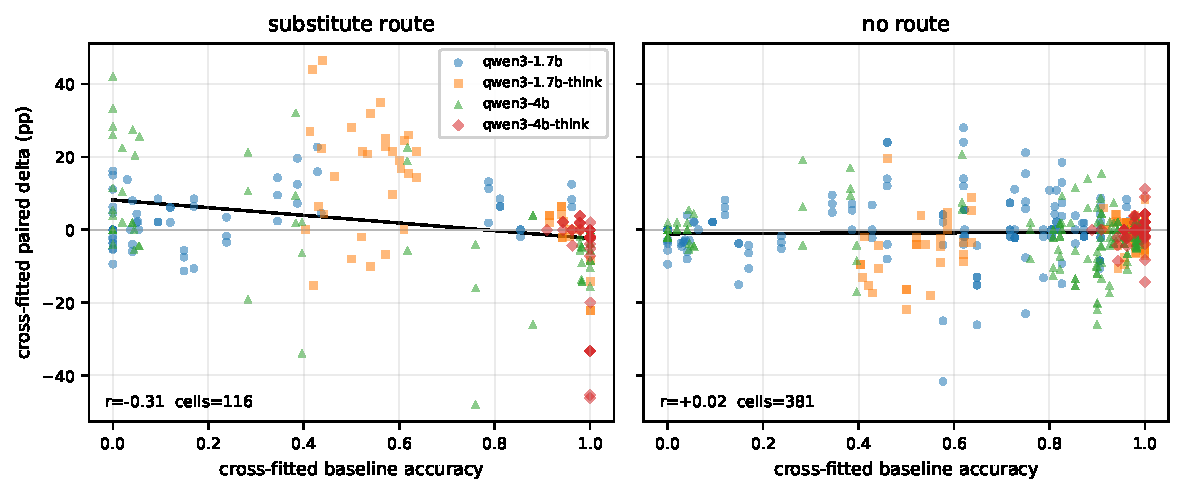
\includegraphics[width=\columnwidth]{../crossfit.pdf}
\caption{Cross-fitted paired effect against cross-fitted baseline accuracy, for
cells where a primer offers a substitute route to the answer (left) and where
it does not (right). Baseline and effect come from disjoint halves of each
cell's graphs.}
\label{fig:crossfit}
\end{figure}

A \emph{cell} is an (arm, task, density, condition) combination with at least
ten usable pairs. Route cells gain where accuracy under \texttt{none} is low
and lose where it is high; no-route cells show no such relation
(Figure~\ref{fig:crossfit}). Because baseline and effect share sampling noise,
we estimate the route $\times$ baseline interaction on cross-fitted halves of
each cell's graphs: $-11.0$ points per unit of baseline, $95\%$ CI
$[-17.1, -5.7]$. A stated answer helps a model that cannot compute the answer
and hurts one that already can.

Two checks bound the claim. First, the relation is \emph{not graded}: within
the $0.10$--$0.90$ baseline window it disappears, so the data support a
floor/ceiling contrast rather than a smooth dependence on competence. Second,
it is not a censoring artifact. The pooled relation covers two tasks, one of
which truncates heavily, so we partition it: over all $232$ route cells
$r{=}-0.308$ with slope $-10.5$ $[-16.6, -5.4]$; over the $168$
\texttt{node\_degree} cells alone $r{=}-0.235$ ($p{=}0.0022$) with slope $-9.1$
$[-21.6, -1.8]$; over the $64$ \texttt{edge\_count} cells $r{=}-0.664$ with
slope $-26.5$. \texttt{node\_degree} truncates on $0$--$1.6\%$ of generations
and carries the relation on its own.

Manipulating difficulty directly reproduces the contrast: for
\texttt{qwen3-1.7b-think} on \texttt{node\_degree}, raising density from
$p{=}.10$ to $.85$ drives accuracy under \texttt{none} down and
\texttt{degree}'s benefit up monotonically, from $+3.1$ to $+34.2$ points.

\section{Length Is an Active Treatment}
\label{sec:length}

Every effect against \texttt{none} decomposes exactly into a length cost and a
content gain,
\[
\underbrace{c - n}_{\text{net}} \;=\;
\underbrace{f - n}_{\text{length}} \;+\;
\underbrace{c - f}_{\text{content}},
\]
with $n$, $f$, $c$ the accuracies under \texttt{none}, \texttt{filler} and the
condition. Over the $90$ cells with an uncontaminated primer and a baseline
between $0.30$ and $0.90$, and correcting across all of them, the content gain
is significant and positive in $29$ cells against $2$ negative, the length cost
is significant and negative in $21$, and the \emph{net} survives in only $11$.
Content helps, length hurts, and they largely cancel.

\texttt{filler} states nothing about the graph, yet significantly reduces
accuracy on \texttt{connected\_nodes} and \texttt{edge\_existence} in both
plain arms --- and across the four arms these are the only non-degenerate
effects that replicate at both model sizes. The cost is not confined to this
corpus: on the published split, \texttt{rwse}, the longest primer, costs
\texttt{qwen3-8b} $13.3$ points of \texttt{edge\_count} accuracy
($36.7\%$ against $50.0\%$, $p<10^{-3}$) and \texttt{qwen3-1.7b} $4.6$ points
($p{=}0.036$).

A primer can also remove an answer rather than change it. Under
\texttt{degree}, \texttt{qwen3-1.7b-think} fails to terminate on $19.2\%$ of
generations against $15.8\%$ under \texttt{none} ($p{=}2.4\times10^{-6}$);
outside \texttt{edge\_count} the rates are $6.9\%$ against $2.6\%$
($p{=}9.2\times10^{-11}$), $130$ new failures attributable to the primer.

\section{What Survives}
\label{sec:survives}

On the main sweep, exactly two primers that do not state the answer beat both
\texttt{none} and \texttt{filler} under a global correction. One is
\texttt{clustering} on \texttt{node\_count}, which Section~\ref{sec:tasks}
disqualifies. The other is \texttt{components} on \texttt{connected\_nodes} for
\texttt{qwen3-4b}: $+9.2$ points over \texttt{none} and $+21.8$ over
\texttt{filler} ($n{=}400$, $p\approx10^{-4}$ for both). Because
\texttt{components} adds nine tokens, it is the only effect here that is
essentially free of length cost, and the gap to \texttt{filler} is mostly
\texttt{filler}'s own damage.

\texttt{clustering} on \texttt{node\_degree} is the effect a dedicated corpus
was built to test. Pooled over $p{=}.35$ and $.50$ with $400$ graphs per
density it gains $+5.9$ points over \texttt{none}
($95\%$ CI $[2.1, 9.8]$), with an independent-seed replication at $+5.5$. Both
the cell and the density window were chosen after the main sweep --- where the
same comparison gives $+3.0$, $p{=}0.26$ --- so the replication, not the
original estimate, is what makes it reportable.

\begin{table}[t]
\centering\small
\setlength{\tabcolsep}{3.5pt}
\begin{tabular}{rrrrrrr}
\toprule
& & \multicolumn{3}{c}{\texttt{qwen3-1.7b}} & \multicolumn{2}{c}{\texttt{qwen3-8b}} \\
\cmidrule(lr){3-5}\cmidrule(lr){6-7}
$n$ & $\bar{d}$ & \texttt{none} & \texttt{clust.} & $\Delta$ & \texttt{none} & $\Delta$ \\
\midrule
$20$ & $8$ & $0.912$ & $0.865$ & $-4.8$$^{*}$ & $0.998$ & $+0.2$ \\
$40$ & $8$ & $0.728$ & $0.770$ & $+4.2$ & $0.995$ & $+0.0$ \\
$80$ & $8$ & $0.645$ & $0.750$ & $+10.5$$^{*}$ & $0.965$ & $-0.8$ \\
$160$ & $8$ & $0.624$ & $0.693$ & $+6.9$$^{*}$ & $0.897$ & $-2.8$ \\
$20$ & $16$ & $0.575$ & $0.740$ & $+16.5$$^{*}$ & $0.985$ & $-0.2$ \\
$40$ & $16$ & $0.398$ & $0.476$ & $+7.8$$^{*}$ & $0.975$ & $+1.0$ \\
$80$ & $16$ & $0.225$ & $0.323$ & $+9.8$$^{*}$ & $0.895$ & $-1.8$ \\
$160$ & $16$ & $0.224$ & $0.211$ & $-1.3$ & $0.802$ & $-4.0$ \\
\midrule
\multicolumn{2}{l}{pooled} & $0.542$ & $0.604$ & $\mathbf{+6.2}$ & \multicolumn{2}{c}{$n{=}3191$} \\
\bottomrule
\end{tabular}
\caption{Fixed-mean-degree sweep: mean degree $\bar{d}$ held at $\approx 8$ or $\approx 16$ while $n$ varies, so density falls as the prompt lengthens. $\Delta$ is \texttt{clustering} against \texttt{none} in points. $^{*}$: exact McNemar surviving Benjamini--Hochberg at $q{=}0.05$ across the eight cells. \texttt{qwen3-8b} is shown as a ceiling control. This corpus has no \texttt{filler} arm, so $\Delta$ is a net effect.}
\label{tab:degfixdeg}
\end{table}


A third corpus, built to separate graph size from answer magnitude, supports it
on a design that played no part in that choice (Table~\ref{tab:degfixdeg}).
Holding mean degree at
$\approx 8$ or $\approx 16$ while $n$ ranges over $\{20,40,80,160\}$,
\texttt{clustering} gains $+6.2$ points over \texttt{none} pooled
($n{=}3{,}191$, $504$ helped against $306$ hurt, $p<10^{-4}$), significant in
six of eight cells after correction, and larger where the answer is larger
($+8.2$ at mean degree $\approx 16$ against $+4.2$ at $\approx 8$). Two caveats
travel with it: the corpus has no \texttt{filler} arm, so this is a net effect
and not evidence that content beats length; and \texttt{qwen3-8b} on the same
grid sits at $0.998$--$0.802$ and shows nothing, which is
Section~\ref{sec:route}'s ceiling result rather than a contradiction.

The same grid dissociates two drivers of difficulty that density confounds.
Holding mean degree fixed, growing $n$ from $20$ to $160$ costs
\texttt{qwen3-1.7b} $29$ points and saturates after $n{=}80$; holding $n$
fixed, doubling mean degree costs $33$ to $42$ points at \emph{every} size. The
magnitude of the answer matters more than the size of the graph.

\section*{Limitations}

The main sweep is two sizes of one model family; the published-split and
fixed-degree corpora add arms but were collected earlier and not
pre-registered. All graphs are Erd\H{o}s--R\'enyi, in which local clustering is
nearly uniform, so \texttt{clustering} carries little node-specific
information --- a likely reason its effect is small. The route split depends on
a threshold and on the $n{=}40$ refit. \texttt{filler} matches
\texttt{clustering}'s length but is much shorter than \texttt{rwse} and
\texttt{all}, so the length control is weakest exactly where length is largest.
\texttt{clustering}'s window was chosen post hoc. Every prompt uses one
encoding, one template and one primer position, with greedy decoding. Several
cells rest on $400$ or fewer instances. We have no mechanism for the
\texttt{clustering} effect: rewiring that drives mean clustering from $0.01$ to
$0.73$ leaves the benefit flat, and a density-prior account predicts a signed
error shift of up to $17$ where the observed shift stays within $0.3$ of zero.
Three further conditions would settle the open questions --- a shuffled-value
placebo stricter than \texttt{filler}, a corrupted primer separating copying
from computation, and a single-fact primer separating interference from route
substitution.

\section*{Conclusion}

Read against the class prior rather than against zero, four of six GraphQA
tasks are compromised at $n{=}40$: two are answered by a constant, one sits
below its prior on both plain arms, and one is scored by a response bias.
Within what remains, a primer that states the requested quantity acts as a
second route to the answer, helping a model at floor and harming one at
ceiling; added text is an active treatment whose cost is the only effect that
replicates across model sizes; and the content effects that survive both
controls are small and confined to two cells. For practice on these tasks and
sizes, priming has near-zero expected value and turns negative as prompts
lengthen, with \texttt{all} and \texttt{rwse} the worst choices on the smaller
arm. For evaluation, a prompt-level graph augmentation should be reported
against a class prior, a length-matched control and a graph-blind solver
together; any one of them alone admits a large effect that is not graph
reasoning.

\section*{Ethics Statement}

This work evaluates open-weight language models on synthetically generated
Erd\H{o}s--R\'enyi graphs. It involves no human subjects and no personal data.
The principal cost is the GPU compute for $217{,}178$ generations.

\bibliography{custom}

\end{document}
